\chapter{Introduction and Motivation}\label{ch:introduction}


Helicopter triggered lightning is a dangerous phenomenon which causes interruptions to helicopter traffic and presents a danger to both pilots and passengers. In 1999 it was estimated that the repair cost due to a helicopter strike was on the order of  ~100k U.S. Dollars (Lunde). The incident rate can be estimated from the Lande-dataset to about 2.05 per year for Norwegian operators in the period 1979-1999 and about 2.5 for UK operators in the period 1990-1999. This would then result in the accumulated economic loss of about ~4.3mil and ~2.5mil for the Norwegian and UK operators respectively.

This potential in economic loss is severe in itself, but added onto this is also the danger helicopter pilots and passengers are put in, when flying in lightning related weather. There are two major helicopter incidents related to lightning in the last 30 years. (1995, and 2001). In the same period there have been one major incident with airplanes among the Norwegian operators (Ref Bodø lufthavn)

Helicopters are a vital part of the transport of personnel to offshore installations along the Norwegian coast. Offshore personnel report fear of being involved in helicopter incidents. They also experience unease from flying in turbulent and bad weather (\cite{wasilewska2019}). These weather types may be causal to incidents, as suggested in earlier work (e.g. \cite{lande1999}; \cite{wilkinson2013}; \cite{smart1997}). It is therefore imperative to exhaust the investigation into the causes of and possible ways to prevent helicopter related incidents. 
Helicopters flying offshore in the higher latitudes of the northern hemisphere are sometimes hit by lightning. This can in various ways be the cause of incidents. These incidents include events when rotors have been destroyed, as in the case of Flight 56 in 1995 (\cite{smart1997}). Sometimes a breakdown of the structural integrity of a rotor by lightning is not discovered right away, but can still be serious. For example, a lightning strike in 1999 is believed to have caused a fatal crash in 2002 (\cite{smart2005}). Incidents of less fatal variety include disruption to electrical equipment (Table 2. \cite{uman2003}). Flying helicopters are in practice only hit by lightning in wintertime, (See Figure \ref{fig:landewilk}) and this phenomenon is referred to as \acrfull{htl} (e.g. \cite{lande1999}; \cite{wilkinson2013}). The triggering refers to the helicopters being hit by lightning in areas where there is little to no lightning activity before the lightning strike. When there is lightning activity present, a helicopter pilot avoids the area (further discussed in section \ref{sec:data}).


\begin{figure}
    \centering
    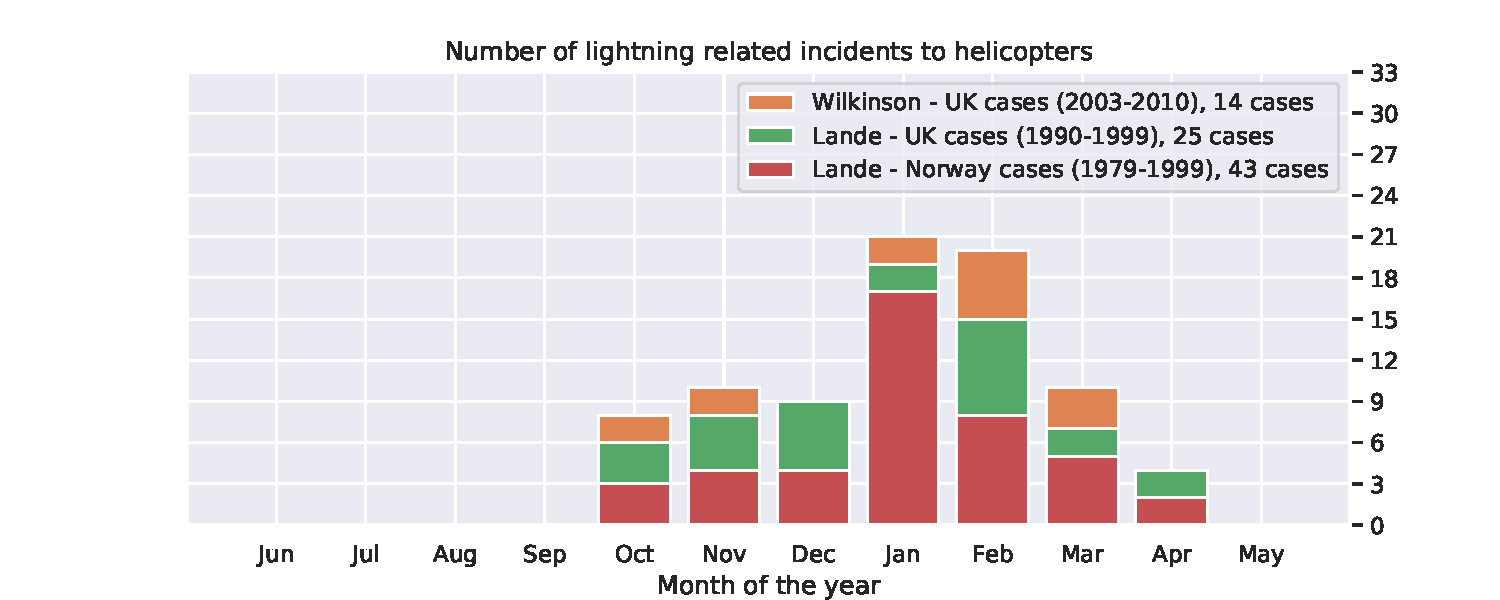
\includegraphics[width=\textwidth]{Figures/yearlydistribution_withoutmine.pdf}
    \caption{Seasonal variation of helicopter cases, showing no cases in May to September. Data is produced from \cite{lande1999} and \cite{wilkinson2013}. Legend notes time-periods and amount of cases in each study.}
    \label{fig:landewilk}
\end{figure}

The study of \acrshort{htl} had its peak around the turn of the century, due to two helicopter incidents related to lightning (1995 and 2002). The 1995 incident was a non-fatal incident. A lightning strike destroyed the main rotor of the helicopter, forcing the pilot to perform a landing in the ocean (\cite{smart1997}). The 2002 incident resulted in eleven fatalities and is believed to have been caused by internal damage to the helicopter's main rotor back in 1997. The initial inspection of the rotor did not uncover any damage, causing the helicopter to be cleared for flight. This initial structural damage later resulted in failure of the main rotor, leading to the crash in 2002 (\cite{smart2005}). These events resulted in practical guidelines to helicopter pilots based on data from earlier incidents (\cite{lande1999}, \cite{hardwick1999}). Furthermore, the UK Met Office added numerical simulation and forecasting to these guidelines, with the introduction of \acrfull{hti}. This provided a more robust warning for helicopter pilots (\cite{wilkinson2013}). Since then, general \acrfull{nwp} forecasts have improved and continue to improve due to better  physical understanding, more and higher quality observations, and increase in available computational power. This thesis aims to improve upon the understanding of the \acrshort{htl} phenomenon by using state-of-the-art model products.

The author makes use of a novel dataset from Avinor containing reported incidents of both  \acrshort{htl} and a similar phenomenon: \acrfull{fwtl}. \acrshort{fwtl} is triggered lightning involving planes and rockets, where the wings are fixed. \acrshort{fwtl}, unlike \acrshort{htl}, is of less danger to both personnel and materials. Fixed wing aircraft are generally hit in the main body. Fuel and vital electronics are also better protected in fixed wing aircraft (\cite{petrov2012}). Helicopters are mainly hit through the rotor into the main body (\cite{lande1999}). Despite this difference in actual risk, both incidents are associated with non-negligible risk, and require thorough inspection of the aircraft after the fact.

To investigate atmospheric conditions during \acrshort{htl} and \acrshort{fwtl} incidents, the \acrfull{era5} dataset is utilized. Also used for this purpose is the operational \acrfull{meps}\footnote{\acrfull{metcoop}}. \acrshort{meps} became available in November 2016, and hence can only provide atmospheric conditions for cases that have occurred since then. \acrshort{meps} provides higher spatial resolution compared to \acrshort{era5}. Further, the \acrshort{meps} ensemble members are evaluated in order to assess if this can provide improved forecast ability for \acrshort{htl}.

These are the research questions this thesis attempts to answer:
\begin{itemize}	
    \item What atmospheric conditions are present for an \acrshort{fwtl}-event and can \acrshort{fwtl} be used as a proxy for \acrshort{htl}? 
    \item Is \acrshort{htl} forecasted well?
    \item In what ways can the \acrshort{htl} forecast be improved?
\end{itemize}

The goal is to improve and strengthen the confidence in the current operational \acrshort{htl} forecast. Also under investigation is an error found in the algorithm used to produce the operational forecast where the accumulated precipitation, and not the intended hourly precipitation, was used in the operational forecast. This lead to a potential over-estimation of risk related to offshore flights.

\section{Layout of the thesis}

The theory builds on the historical context, but also introduce the physical mechanisms of lightning-producing storms. In section ... this is used to investigate the physical mechanisms believed to be present in a winter-lightning situation. This again is related to \acrfull{htl} in section ... and how a short discussion about the challenges related to forecasting this phenomenon is had.

The method chapters discussed the data and methods used in this thesis. The first section (sec....) is dedicated to detailing the models producing the data used. Section ... then details the dataset received from Avinor. Lastly section ... describes the methods used in this thesis, ranging from the already implemented algorithm, to statistical sizes used in this thesis.

The results chapter starts off with investigation into the temporal and spatial spread of the cases of lightning incidents to aircraft. This is then followed by a section on the atmospheric conditions during these cases. These atmospheric conditions are then investigated in the operational model. Lastly a preliminary investigation into usage of EPS is performed.




